\chapter{3D case}
\label{chapter:3d}

% {{{1 PROBLEM
\section{Problem}

In this part, we will focus on point clouds in 3D that sample a surface.  We can
do the same work as the one done in 2D that is to say smooth the point cloud
using a mean curvature flow approach: compute the gradients of the volume of a
union of balls. The computation of the volume has already been done in
\cite{cazals2011computing}. But, since the expected results are the
same (see Chapter \ref{chapter:theory}): smoothing of the point cloud and a
discretization of the mean curvature flow, we preferred to focus to an other
kind of flow: an anisotropic one.

The idea of this flow is to replace the union of balls with a union of convex
polyhedra. The choice of the polyhedron will directly influence the directions
in which the points will be moved.

For doing that, we will replace the euclidean ball $ B(0, r) $ with a convex
polyhedron which can be considered as the unit ball for a certain norm $ N $
which we call a polyhedral norm (see Section \ref{sec:polyhedral-norm}). Then,
the formula \ref{eqn:area-union-balls} will be valid if we replace $ B(p, r) $
with $ B_N(p, r) $ and $ V $ by $ V_N $ (the Voronoi diagram computed for the
norm $ N $) only if the points are in general position. See Appendix
\appendixref{appendix:voronoi-polyhedral-norm} for a study of some properties of
the Voronoi diagram for a polyhedral norm. Indeed, see Figure
\ref{fig:3d-voronoi-cube} for a look at a particular case where the chosen
polyhedron is a cube (norm $ L^\infty $). We see that if we chose two aligned
points, the bisectors are not lines anymore and so the Voronoi diagram does not
decompose the plane anymore. Furthermore, the computation of the Voronoi cells
for a polyhedral norm is a tough work (see \cite{ma2000bisectors} for a thorough
study).

\begin{figure}[h]
    \centering

    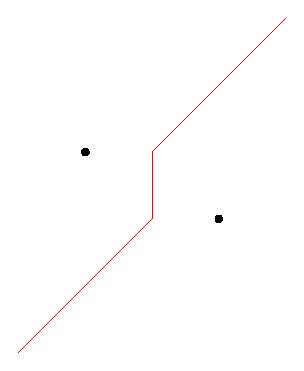
\includegraphics[scale=0.5]{3d/voronoi-cube-non-aligned}
    \hspace{2cm}
    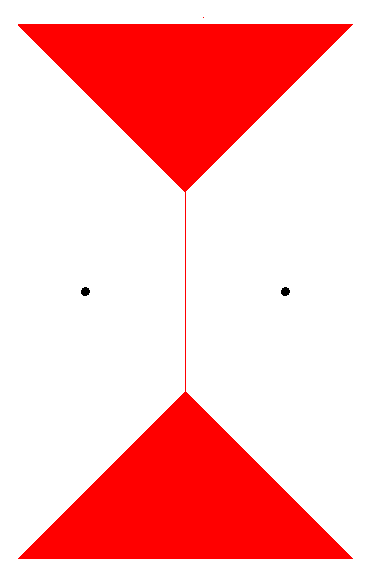
\includegraphics[scale=0.5]{3d/voronoi-cube-aligned}
    \caption{Bisector for the $ L^\infty $ norm: two non aligned points / two
        aligned points}
    \label{fig:3d-voronoi-cube}
\end{figure}

That's why we do not use the Voronoi diagram for the norm $ N $ but the standard
Voronoi diagram for the $ L^2 $ norm. Instead of computing the intersection $
V_N(p, P) \cap B(p, r) $ we compute $ V(p, P) \cap B(p, r) $. In order to
compute this intersection, we used different methods: a naive one, one based on
inclusion-exclusion formula. We will see that both of these methods are
approximated ones. There is also one method which is exact but we did not have
the time to implement it in our internship, it is based on 3D arrangements and
overlays.

Firstly, we will explain what we call the naive method. Secondly, we will study the
inclusion-exclusion formula. Then, we will talk about the choices we made for
the implementation and finally, we will run experiments to validate our
expectations.

% {{{1 POLYHEDRAL NORM
\section{Polyhedral norm}
\label{sec:polyhedral-norm}
A polyhedral norm is a function $ N $ defined as the following:

\begin{equation}
    \forall x \in \mathbb{R}^d,~ N(x) = \max_{i} (x | v_i)
\end{equation}

where the $ v_i $ are given vectors from $ \mathbb{R}^d $.

This definition implies that the unit ball for the norm $ N $ is a
polyhedron.Indeed, if $ x \in B_N(0, 1) $, then :

$$ N(x) \leq 1 \Longleftrightarrow \forall i,~(x | v_i) \leq 1 $$

So, the unit ball is defined by linear constraints. Thus, it is an intersection
of halfspaces and so is a convex polyhedron $ K $ The vectors $ v_i $ are the
normal vectors to the facets of $ K $. We will denote by $ B_K(0, 1) $ the unit
ball defined by the convex polyhedron $ K $.

% {{{1 VOLUME OF A UNION OF POLYHEDRA
\section{Volume of a union of polyhedra}

In this section, we will show how to compute an approximation of the volume of
a union of polyhedra using two different methods: a naive one and one based on
inclusion-exclusion formula.

% {{{2 NAIVE METHOD
\subsection{Naive method}
We want to compute :

\begin{equation}
    Vol(\bigcup_{p \in P} B_N(p, r)) = \sum_p Vol(\bigcup_p B_N(p, r) \cap V(p, P))
\end{equation}

The idea of this method is to approximate $ Vol(\bigcup_p B_N(p, r) \cap V(p,
P)) $ by $ Vol(B_N(p, r) \cap V(p, P)) $. Then, we just have to compute the
intersection of halfspaces (see Section \ref{sec:3d-implementation} for
details). It is an approximation because, for example, if we want to compute the
perimeter of the boundary of squares in 2D, there is a difference between what
we want to compute and what we actually compute is (see Figure
\ref{fig:3d-inclusion-exclusion-squares}).

\begin{figure}[h]
    \centering

    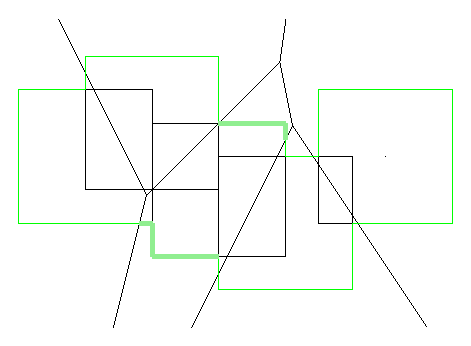
\includegraphics[scale=0.8]{3d/3d_perimeter_squares_truth}
    \hspace{2cm}
    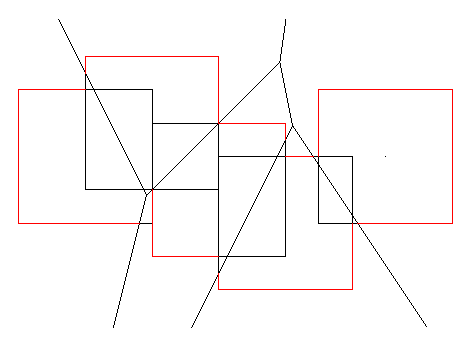
\includegraphics[scale=0.8]{3d/3d_perimeter_squares}
    \caption{In green, what we want and in red what we actually compute}
    \label{fig:3d-inclusion-exclusion-squares}
\end{figure}

There is a small difference between the two: our computation is just
an approximation.

% TODO: explain approximation

% {{{2 INCLUSION-EXCLUSION FORMULA
\subsection{Inclusion-exclusion formula}
% TODO

The inclusion-exclusion formula is a well known formula which describes the
indicator function of a union of sets: given a finite number of sets $ A = \{
A_1, \ldots, A_N \} $, we have:

\begin{equation}
    \indicator{\bigcup A_i} = \sum_{\emptyset \neq X \subseteq A} (-1)^{card X -
        1} \indicator{\bigcap X}
\end{equation}

This formula can also be expressed using the notion of nerve as shown in
\cite{attali2007inclusion}. We define the nerve of $ A = \{ A_x, x \in X \} $
to be the graph where an edge exists between $ x $ and $ y $ if $ A_x \cap A_y
\neq \emptyset $. Then, we can write the inclusion-exclusion formula as:

$$ \indicator{\bigcup A_x} = \sum_{\sigma \in Nerve(A)} (-1)^{\dim \sigma}
\indicator{\bigcap \sigma} $$

$ \sigma $ represents any simplex in the nerve. Its dimension is defined as: $
\dim \sigma = card \sigma - 1 $.

If we consider a union of polyhedra, we can write a similar formula:

\begin{equation}
    \indicator{\bigcup B_N(p, r)} = \sum_{\sigma \in Nerve(B)} (-1)^{\dim \sigma}
    \indicator{\bigcap \sigma}
    \label{eqn:incl_excl_simplices}
\end{equation}

where $ B $ is the collection of all the balls $ B_N(p, r), p \in P $.

Now, since the nerve can be a really big object, we want to restrict the
computation to what we call the $\alpha$-complex of a set of points:

\begin{definition} The $\alpha$-complex of a set of points $ X $ denoted by $
    Del(X, \alpha) $ is a subset of the Delaunay triangulation. For each simplex
    of the Delaunay triangulation, we can associate to it a characteristic
    radius: the radius of the smallest empty circle containing the simplex.

    Now, the $\alpha$-complex contains all the simplices of the Delaunay
    triangulation whose characteristic radius is smaller than $\alpha$.
\end{definition}

Now, we can ask if the formula \ref{eqn:incl_excl_simplices} is still valid if
we replace $ Nerve(B) $ by $ Del(P, r) $.

A question we can ask is the following: is the inclusion-exclusion formula still
valid if we replace $ Nerve(B) $ with $ Nerve(\{ B_N(p, r) \cap V(p, P), p \in
P\}) $ ?

If we want to prove this assertion, we may use the technique used to prove the
inclusion-exclusion formula for a union of balls. The proof starts by defining
the subcomplex $ L_p $ induced by a vertex $ p $.  We consider all the
polyhedrons that contains $ p $ and we construct the nerve of it. Formally, $
L_p = Nerve(\{ B_N(x, r), p \in B_n(x, r)\}) $.

Then, when we evaluate the indicator function at $ p $ of the union, we can
decompose it in two parts: simplices of $ L_p $ and the other ones.

\begin{align*}
    \indicator{\bigcup B_N(p, r)}(p) &= \sum_{\sigma \in L_p} (-1)^{\dim \sigma}
    \indicator{\bigcap \sigma}(p) + \sum_{\sigma \notin L_p} (-1)^{\dim \sigma}
    \underbrace{\indicator{\bigcap \sigma}(p)}_{= 0 \text{ since } p \notin
        \sigma} \\
    &= \sum_{\sigma \in L_p} (-1)^{\dim \sigma} \\
    &= \chi(L_p)
\end{align*}

Here, $ \chi $ is the Euler characteristic of $ L_p $.

Now, if we show that $ L_p $ is contractible (can be continuously deformed to a
point), we will get $ \chi(L_p) = 1 $. Obviously, we also have $
\indicator{\bigcup B_N(p, r)}(p) = 1 $ and we will conclude that the formula
\ref{eqn:incl_excl_simplices} is true.

We can use this argument to generalize this formula. If we suppose that there
exists $ r, r' $ such that: $ B(p, r) \subseteq B_N(p, r) \subseteq B(p, r') $,
then we have: $ K_p \subseteq L_p \subseteq K'_p $ where $ K_p $ (resp. $ K'_p $)
is the induced subcomplex of $ p $ in the simplicial complex defined by all the
balls $ B(p, r) $ (resp. $ B(p, r') $), $ p \in P $.

Then, we know that $ K_p $ and $ K'_p $ are either empty or contractible. If
we are able to deduce that $ L_p $ is either empty or contractible, then the
proof is done.

% TODO: finish the proof

% {{{1 IMPLEMENTATION DETAILS
\section{Implementation details}
\label{sec:3d-implementation}

We used the same libraries as in the 2D case except for the rendering part, in
2D, we used custom \texttt{QWidget}. In this part, we choose to use an
\texttt{OpenGL} based renderer: \texttt{QGLViewer}.

For the first method, the Voronoi diagram is represented implicitly as a list of
halfspaces (the planes defining the boundary of the cell). Halfspaces are
computed using the Delaunay triangulation. Since the order traversal of the vertices
of the Delaunay triangulation is not, in general, be the same as the insertion
order, we need to associate an index to a point (using a simple
\texttt{std::map}).

For the two methods, we needed a way to compute intersection of halfspaces: for
the first one, we need to compute the intersection of a Voronoi cell and a
convex polyhedron and for the second one, we need to compute intersections of
convex polyhedra.

A convex polyhedron $ K $ represents the unit ball for the polyhedral norm
defined by $ K $. It is represented as a list of the normal vectors for each
facet. Using this representation, we can compute the translated polyhedron $
B_K(p, r) $ for a point $ p $ by saying that it is the intersection of the
following halfspaces: $ \forall n,~ n_x x + n_y y + n_z z - (p | n) - r \leq 0 $
where $ n $ is a normal vector of a facet.

In order to construct this intersection, we used the duality which allows us to
replace the computation of the intersection by the computation of the convex
hull (see \cite{preparata1979finding}) of the dual points: at each halfspace, we
can associate a dual point and conversely.

Programmatically, we compute this intersection in the following manner:
\begin{enumerate}
    \item Compute the dual points by remembering which point is associated to
        which plane
    \item Compute the convex hull of these points, it gives us a dual
        polyhedron. At each vertex, we associate the corresponding primal plane.
    \item To compute the primal polyhedron, we first compute the primal vertices
        which are the dual of the dual facets: each dual facet has at least 3
        vertices. We know the corresponding primal planes for these vertices.
        Then, the corresponding primal vertex is the intersection of these 3
        planes. Then, the primal facets are constructed by circulating around
        the dual vertices. Each time there is an edge between two dual vertices,
        there is an edge between the two corresponding primal vertices.
\end{enumerate}

See Appendix \appendixref{appendix:code-intersection} for a simplified version of this algorithm:

Let's now explain in more details the integration of the automatic
differentiation tool.

\texttt{CGAL} has the particularity to make easy for the programmer to change
the number type by using the concept of a \emph{Kernel}. A \emph{Kernel} is a
class that describes how numbers are stored in memory, how we can construct
things (like points, planes, bisectors...) and how to evaluate predicates on
objects (collinearity test, coplanarity test, greater distance to a plane...).
There are multiple predefined kernels but we will quickly talk about two
particular ones. \texttt{Simple\_cartesian<NT>} is the most basic one: a number
will just be represented by \texttt{NT} and so it has inexact predicates
evaluation and inexact constructions.

\texttt{Exact\_predicates\_inexact\_constructions\_kernel} (in short
\texttt{Epick}) is a Kernel which use a technique called \emph{filtering} to
ensure the predicates are always evaluated in an exact manner. In short, the
predicate is the first evaluated in an inexact way using interval arithmetic.
Then, if the resulting interval does not contains zero, then a result can be
returned. Otherwise, the computation is done again using exact arithmetic which,
in all the cases, will give back an answer.

This is precisely the technique we used to use Automatic Differentiation with
\texttt{CGAL}, we used the Kernel: \texttt{Simple\_cartesian<AD>} where
\texttt{AD} is a class with two members: a value and a vector of derivatives.
It implements all the classical arithmetic operations and some mathematical
functions (\texttt{sqrt}, \texttt{atan2}...).

For example, the implementation of \texttt{sqrt} for AD looks like this:
\lstinputlisting[language=C++]{code/sqrt_AD.h}

The choice of \texttt{Simple\_cartesian} may seem inappropriate because the
constructions are inexact but it is enough for our applications.

Now, for the second method, we also needed a way to compute the $\alpha$-complex
of a set of points. This has been done using the \texttt{Alpha\_shapes\_3} class
of \texttt{CGAL}.

% TODO

% {{{1 EXPERIMENTS
\section{Experiments}

% TODO

We compare the two different methods using various polyhedrons as base and
various point clouds.

We can choose for the polyhedron a sufficiently discretized sphere. We expect
the result to be the same as in the 2D case: gradients oriented like the outward
normal with a norm proportional to the mean curvature.

The figures \ref{fig:3d-mean-curvature-sphere-cube} give an example where the
point cloud is a sphere and the polyhedron is a cube.

\begin{figure}[h]
    \centering
    \begin{minipage}{0.32\linewidth}
        \centering
        \includegraphics[scale=0.3]{3d/sphere-polyhedron-200}
        \subcaption{Discretized sphere with 200 planes}
    \end{minipage}
    \begin{minipage}{0.32\linewidth}
        \centering
        \includegraphics[scale=0.3]{3d/sphere-1000}
        \subcaption{Initial point cloud: 1000 points on a sphere}
    \end{minipage}
    \begin{minipage}{0.32\linewidth}
        \centering
        \includegraphics[scale=0.3]{3d/sphere-sphere-1000-05}
        \subcaption{Gradients of the volume}
    \end{minipage}
    \caption{Sphere / cube}
    \label{fig:3d-mean-curvature-sphere-cube}
\end{figure}
We remark that the gradients are oriented like the outward normals.

We also did some experiments for checking the convergence of the flow.

The figures \ref{fig:3d-flow-sphere-cube} give an example where the point cloud
is a sphere and the polyhedron is a cube.

\begin{figure}[h]
    \centering
    \begin{minipage}{0.32\linewidth}
        \centering
        \includegraphics[scale=0.4]{3d/sphere-cube-0}
        \subcaption{Initial sphere with 1000 points}
    \end{minipage}
    \begin{minipage}{0.32\linewidth}
        \centering
        \includegraphics[scale=0.4]{3d/sphere-cube-10}
        \subcaption{After 10 iterations}
    \end{minipage}
    \begin{minipage}{0.32\linewidth}
        \centering
        \includegraphics[scale=0.3]{3d/sphere-cube-cube}
        \subcaption{Shape of the cube}
    \end{minipage}

    \caption{Flow of a sphere under a cube}
    \label{fig:3d-flow-sphere-cube}
\end{figure}

% TODO:
% - description des différentes méthodes + comparaison
% - résultats

% vim: set spelllang=en filetype=tex :
